\clearpage
\section{Introduction}\label{sec:intro}
This project is about developing a design, simulation and optimization tool for casual users to build their own multicopters. Initially it was a research project led by the Computational Fabrication Group at MIT CSAIL in 2015. After we published a paper~\cite{du2016} we got inquiries from many different sources so we decided to release our source code for the benefits of both the research and hobbyist communities.

For those who have read that paper, please note that the code here only covers a subset of our implementation in the paper, as we are still in the middle of cleaning it up. We expect to release all features in the next version ($0.3$).

\subsection{Problem Definition}
Suppose you are a drone hobbyist who wants to have more fun in building your own copters. Below is a list of questions you might want to ask yourself before you start:
\begin{itemize}
\item What components to use: This includes choosing the right material to build the frame (carbon fiber, wood, plastic, etc), picking the proper motors and propellers, selecting a good battery, and many more.

\item How to assemble them: You may want to follow standard designs like a quadcopter, or try some fancy configurations like a tricopter, or even come up with your own, unique configuration, like the bunny-shaped example in our paper.

\item How to control its flight: Normally, you can find a mature controller design for classic quadcopters, which is typically a multi-layer PID controller, for example. If you want to have more degrees of freedom in our design, you probably need to develop your own controllers, or at least spend some time modifying and tweaking an existing controller from similar models.

\item How to verify the design: Crashing a real drone is a huge pain and loss, both psychologically and financially. This is why people turn to software simulation for help. Ideally, it should verify both the geometry and controller accurately, and it should be embedded in the design loop to allow for interactive changes.
\end{itemize}
Obviously, this is a very involved process requiring a diverse set of skills, including mechanical engineering, electrical engineering, programming, control theory, and hands-on experience in building stuff. The goal of our software is to expedite and simplify this process by hiding low level technical details so that people can focus more on expressing and exploring the design space. Specifically, we provide:
\begin{itemize}
\item A dataset of standard components that users can freely choose from and assemble by defining their own scripts.
\item An easy-to-use user interface to explore designs in an interactive way.
\item An automatically determined LQR controller that is generalizable for most existing designs we have seen so far.
\item A real-time simulation tool seamlessly embedded in the design loop to visualize results instantly.
\end{itemize}

Please keep in mind that this software is not meant to replace all the work involved in building a customized drone. You are expected to do your own measurement, or at least give a rough estimation of the physical properties of the motors, propellers and batteries. The output of our software is a hardware specification you can follow, but of course you still need to fabricate or buy these components and assemble them manually. Finally, we include a controller in the solution, but uploading it into your own flight controller board is beyond the scope of this software. You are expected to have a working knowledge of the flight controller (both the hardware and software) you plan to use, and be comfortable with modifying its code to include a new controller.

\subsection{Inputs and Outputs}
The input is an XML file that defines the initial copter design. It provides a straightforward way to format all the essential information needed in the software. We provide a few sample XML files for you to start with, including a standard quadcopter, a V-Tail quadcopter, a Y6 hexacopter and a ``pentacopter'' with 5 motors. Section~\ref{sec:file} provides a detailed explanation on the file format for your reference.

The output includes a hardware fabrication plan and a matrix of control parameters. This plan provides hardware specifications like rotor positions and tube sizes so that by following it you should be able to replicate your virtual design. The control parameters fully determine the LQR controller, and if you are familiar with your flight software it should be fairly straightforward to translate them into the code on board.

\subsection{An Example}
As a concrete example, here we demonstrate how our software can be used to help design and simulate a V-Tail copter~\ref{fig:vtail_ui}. When the window first pop up, you will see a V-Tail model centered on screen, and a few windows floating on both sides. Below we will briefly explain the user interface and show a simple design and simulation loop. A more thorough description can be found in Section~\ref{sec:ui}.
\begin{figure}[!htb]
  \centering
  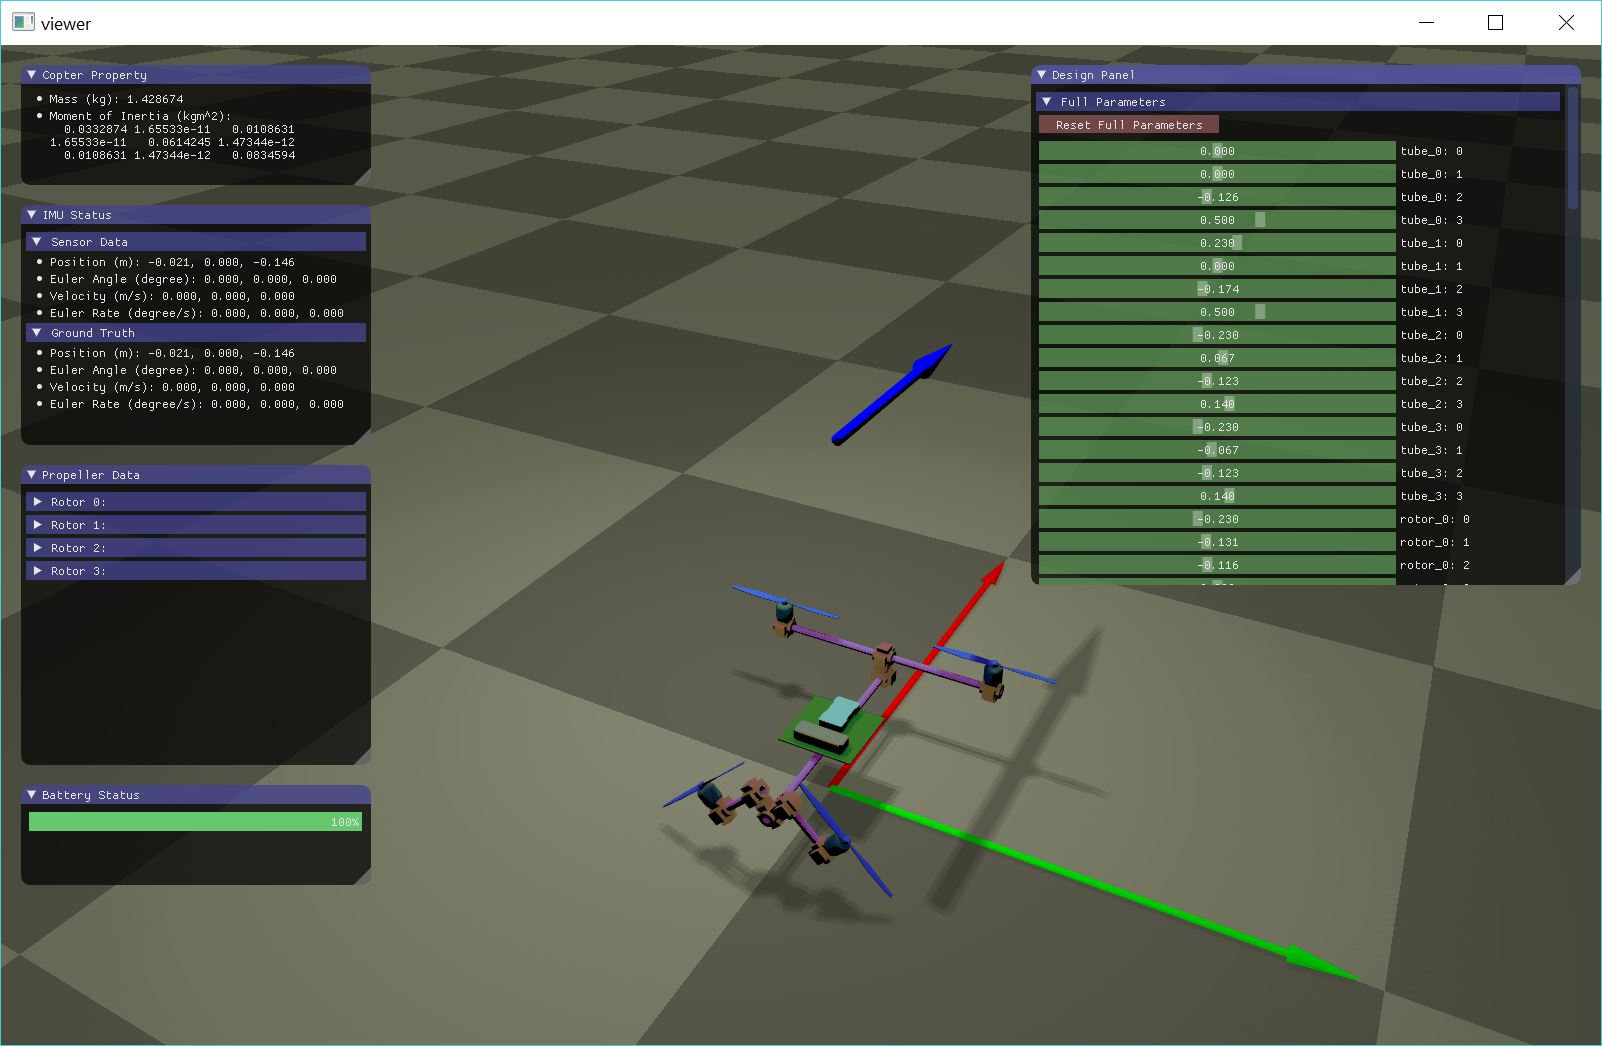
\includegraphics[width=0.9\linewidth]{vtail_ui}
  \caption{Loading the given V-Tail design into our software. The left windows show the current status of the copter, and the right panel allows you to freely explore and simulate different designs.}
  \label{fig:vtail_ui}
\end{figure}

\subsubsection{Basic Information}
On the top left you will find a window named ``Copter Property''. This consists of the mass and inertia of the current design, both of which are computed by collecting information from each component in the XML file. Later, when you change your design, this panel will get updated automatically.

\subsubsection{Design Panel}
On the right there is a long window for you to explore more design possibilities. In our software a copter is parametrized, meaning its shape is fully determined by a list of underlying parameters. These include the length of a tube, 3D position of a connector, height of a plate, and so on. Certain constraints are imposed to ensure the parameters are feasible. For example, a motor should always be attached to a connector instead of freely floating in the air. Please refer to Section~\ref{sec:file} for more details about parameters in each component and its constraints.

\paragraph{Full Parameters} The first panel named ``Full Parameters'' lists a union of parameters from each component. When you use a slider, it specifies a desired value of that particular parameter. A linear least square problem is then solved to find parameters that respect all constraints and are closest to the desired value. Once a solution is found, the copter design in the middle gets updated automatically, and usually in real time (Figure~\ref{fig:vtail_change_full_param}).
\begin{figure}[!htb]
  \centering
  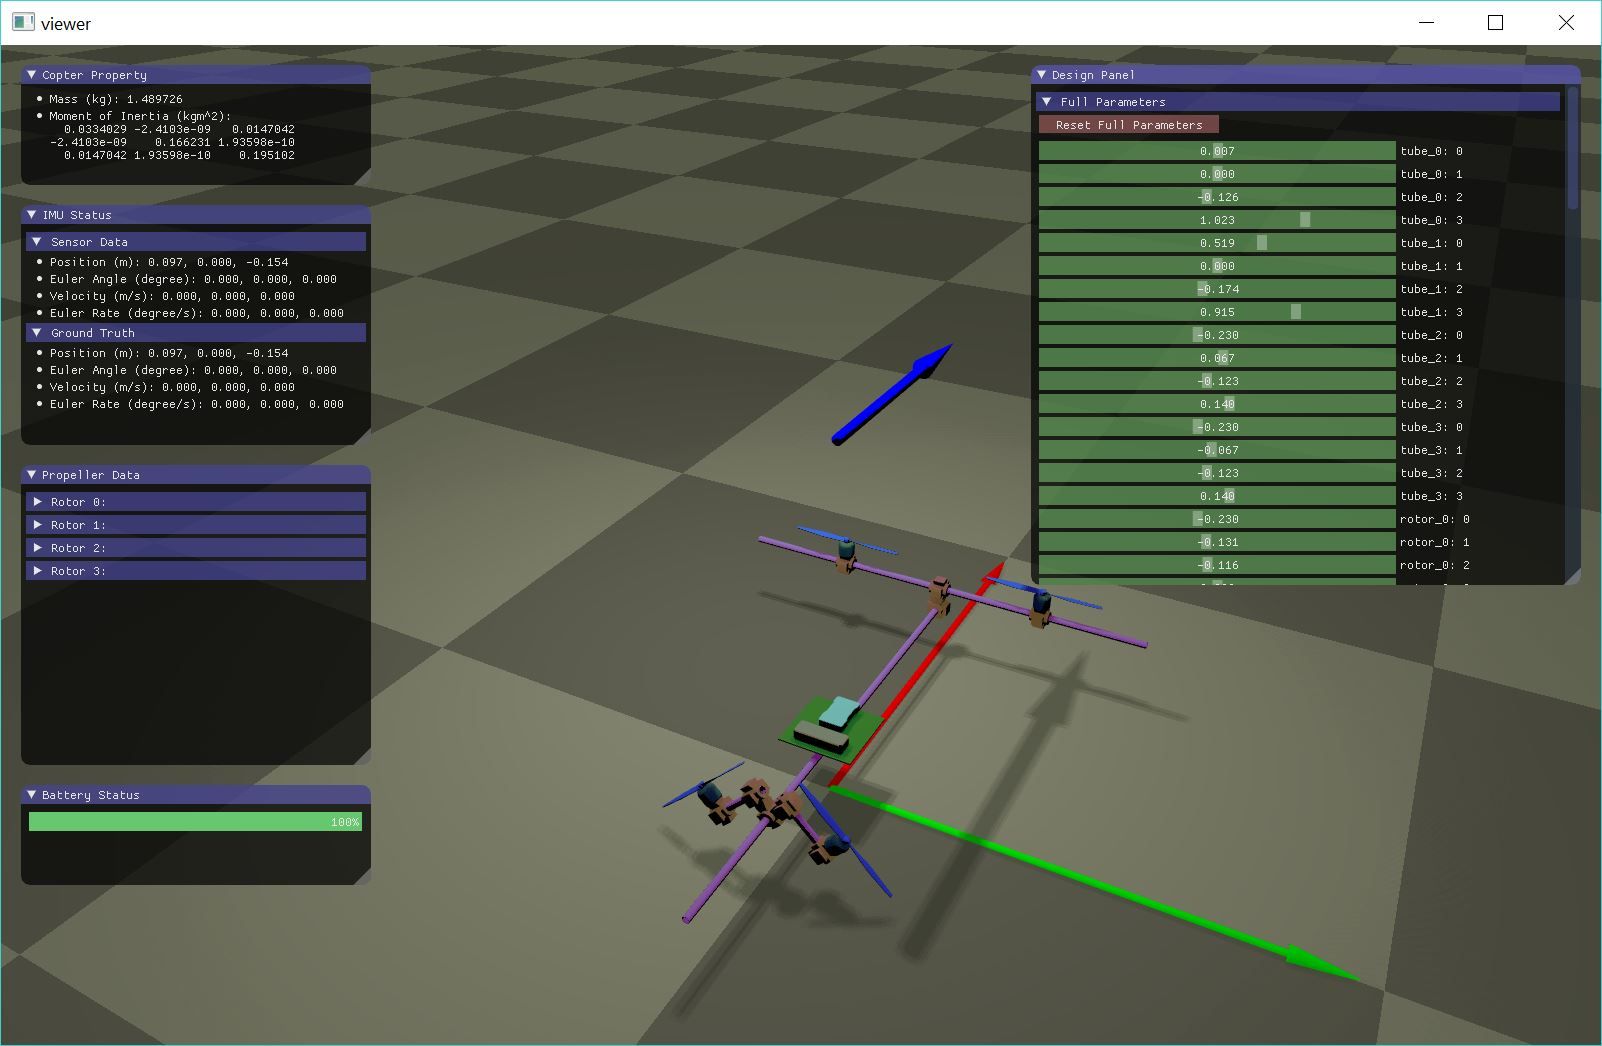
\includegraphics[width=0.9\linewidth]{vtail_change_full_param}
  \caption{By adjusting the full parameters, we elongate two tubes and push the front rotors farther from the center.}
  \label{fig:vtail_change_full_param}
\end{figure}

\paragraph{Reduced Parameters} A copter design consists of up to hundreds of parameters. However, most of them are over constrained by the relative locations between different components. As a result, we also provide a panel to manipulate the reduced parameters, which is usually less intuitive but has way fewer degrees of freedom. Technically, this is done by replacing the linear equality constraints with vectors in its null space.

When you slide the reduced parameters, you may notice the background color sometimes changes between green and red. This color indicates the current parameter is feasible (green) or breaks certain constraints (red). If you slide it into red, the new value will be rejected and the current design remains unchanged.

Finally, there is a ``Reset'' button in both ``Full Parameters'' and ``Reduced Parameters'' windows. Simply clicking it will reset the copter to its original design.

\subsubsection{Simulation}
Once you are satisfied with the current copter, scroll down in the design panel, and you will find a ``Simulate'' button. Clicking it will trigger the software to compute a proper LQR controller and start simulating a virtual flight (Figure~\ref{fig:vtail_simulate}). Press this button will invalidate the ``Full Parameters'' and ``Reduced Parameters'' windows. The button itself will change to ``Reset'' so that you can switch back to the design process if more iterations are needed.
\begin{figure}[!htb]
  \centering
  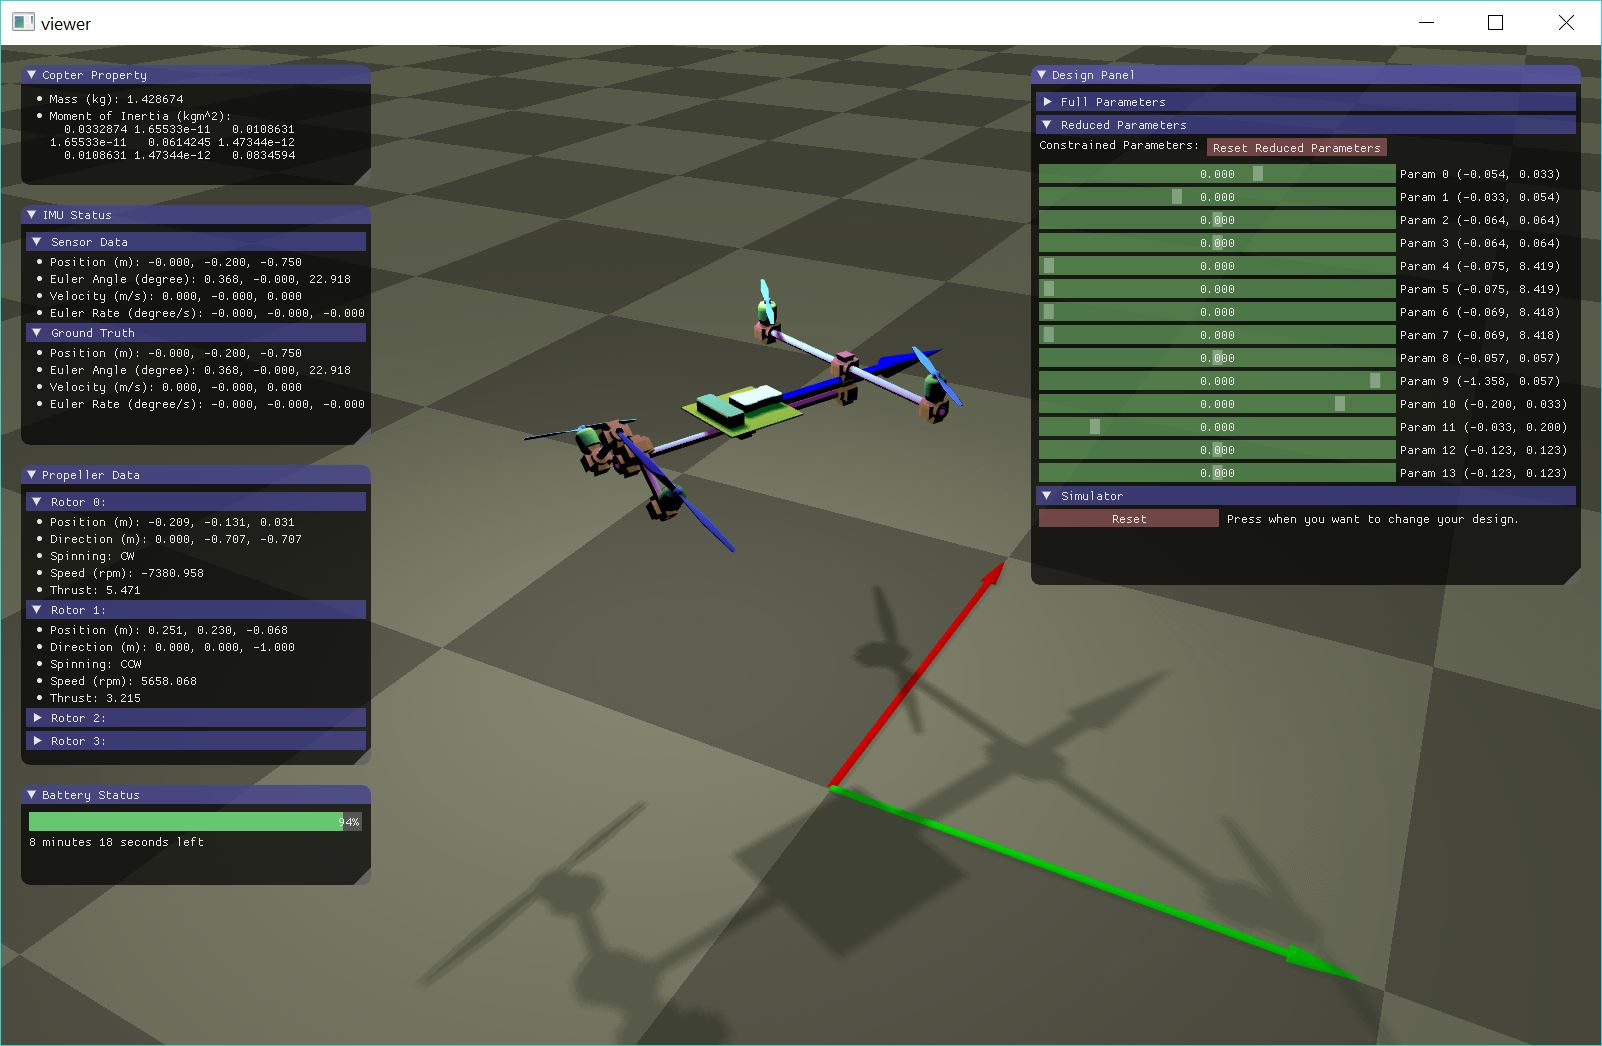
\includegraphics[width=0.9\linewidth]{vtail_simulate}
  \caption{The V-Tail quad is executing a virtual flight in simulation. The copter is trying to follow the position and heading specified by the blue arrow.}
  \label{fig:vtail_simulate}
\end{figure}

During the flight, this copter will try to track the blue arrow as close as possible. Specifically, it interprets the tail as the target position and the arrow as the desired heading. You can use the four arrow keys plus `a', `d', `w' and `s' to adjust the blue arrow and guide your copter to a desired position. You can also change the camera view by mouse gestures like scrolling or panning.

\subsubsection{Flight Status}
On the middle and lower left we provide you more windows to monitor the current status of your copter during flight. The ``IMU Status'' window displays the ground truth position, velocity, rotation and angular rates as well as their readings from the sensor. Currently no noise is added to the sensor so it gives perfect data identical to the ground truth.

Below the sensor data is the ``Propeller Data'' window. Here you can monitor the spinning rate and direction of each propeller. This window also includes basic information like the position and direction of each rotor.

Finally, a ``Battery Status'' window is on the lower left. This shows an estimation of the battery life by summing up the current flowing to each rotor. The progress bar will turn red when the battery is about to drain.

The remaining sections in this document are organized as follows: Section~\ref{sec:install} provides a step-to-step tutorial about downloading, compiling and running our code on different platforms (Windows, Linux, and macOS). Section~\ref{sec:ui} is a detailed description of our user interface, where you can learn more about the design and simulation features. Finally, if you want to try our own copter in our software, Section~\ref{sec:file} gives you a thorough description of the XML file format used to define a copter design. Follow that section to learn how to write your own XML file and load it into our software design and simulation loop.